\section{\ttt{2D} classification}
 \begin{figure}[H]
  \centering
  \captionsetup{width=.8\linewidth} 
  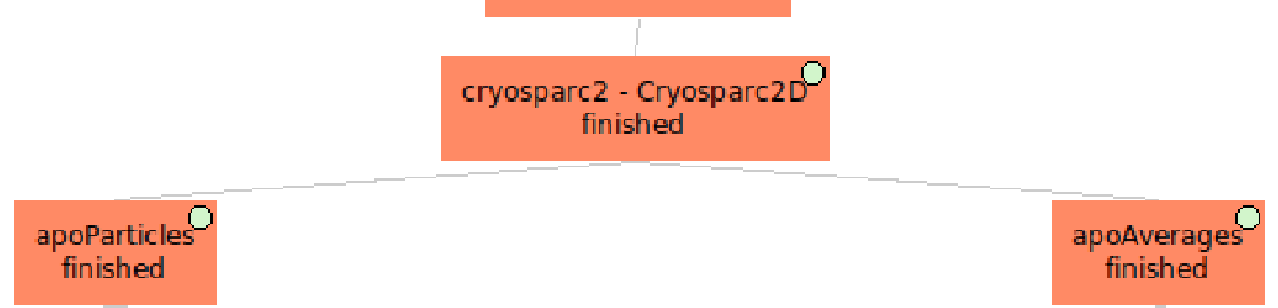
\includegraphics[width=0.95\textwidth]
  {{images/workflow_4_b.pdf}}
  \caption{\ttt{2D} classification workflow.}
  \label{fig:workflow_4_b}
  \end{figure}
The next step in image processing involves the \ttt{2D} classification of the particle images to group similar ones. This process can serve as an exploratory tool of your data and might also be used to throw away bad particles. In addition, by overlapping similar images we can obtain the average images or \ttt{2D} classes. Since these classes are the projections of the 3D object that we try to reconstruct, they can also be used in the reconstruction of the \ttt{3D} object.\\

Although there exist several \ttt{2D} classification algorithms, in this tutorial the \ttt{2D} classes will be created with the $cryoSPARC$ \citep{punjani2017cryosparc} \ttt{2D} classification method \citep{punjani2016building}, integrated in the protocol \scommand{cryosparc2- 2d classification}. We used the subset of particles previously selected as input. The \ttt{2D} classification parameters can be observed in the central tap of the protocol form in the \ffigure{fig:cryosparc2_second_tap}. Remark that we choose in advance the number of classes, 16 in this case.

\begin{figure}[H]
  \centering
  \captionsetup{width=.8\linewidth} 
  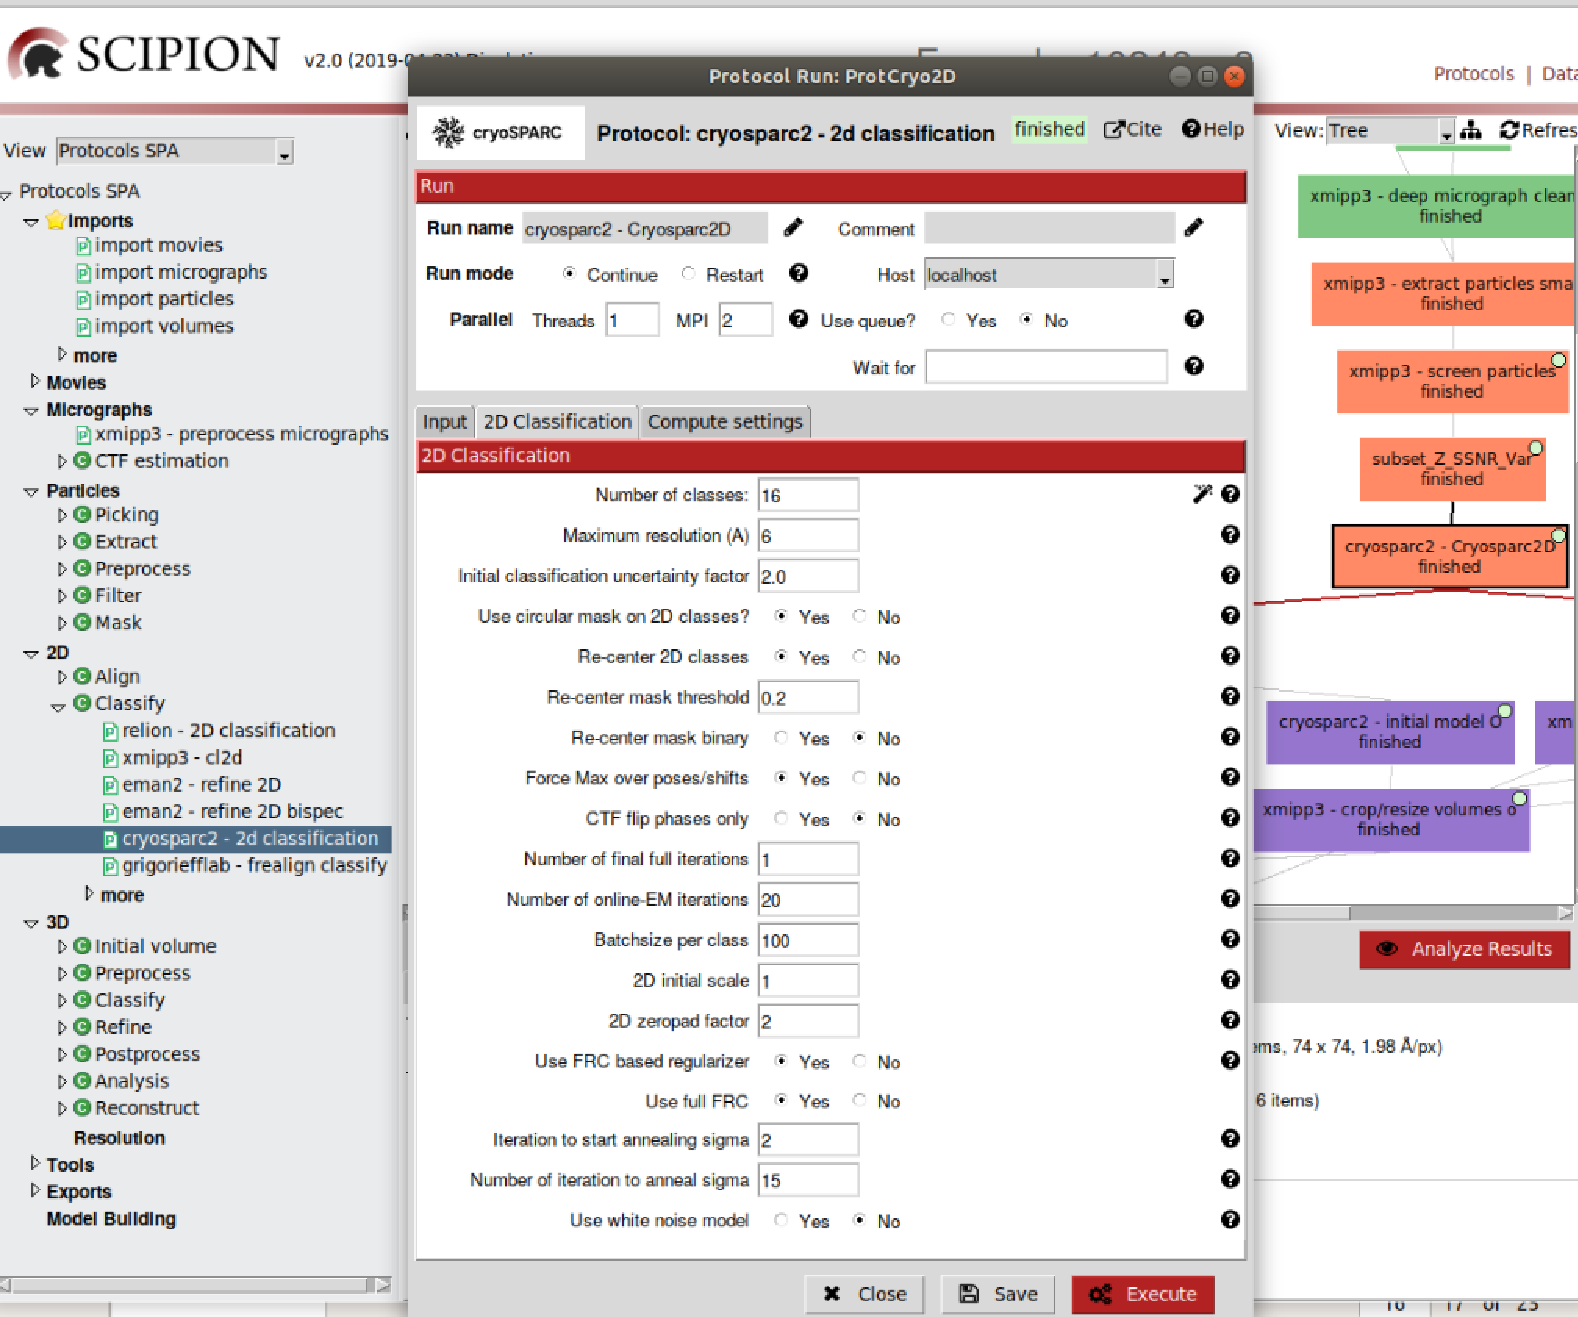
\includegraphics[width=0.95\textwidth]
  {images/cryosparc2_A.pdf}
  \caption{Filling in the second tap of the protocol \scommand{cryosparc2-2d classification}.}
  \label{fig:cryosparc2_second_tap}
  \end{figure}
  
After running the protocol, particle classes can be visualized selecting any of the two options of the menu opened with \scommand{Analyze Results}, the common \scipion viewer or the $cryoSPARC$ GUI. The final number of classes also appears in the Summary output detailed in the \ffigure{fig:cryosparc2_2branches}.

\begin{figure}[H]
  \centering
  \captionsetup{width=.8\linewidth} 
  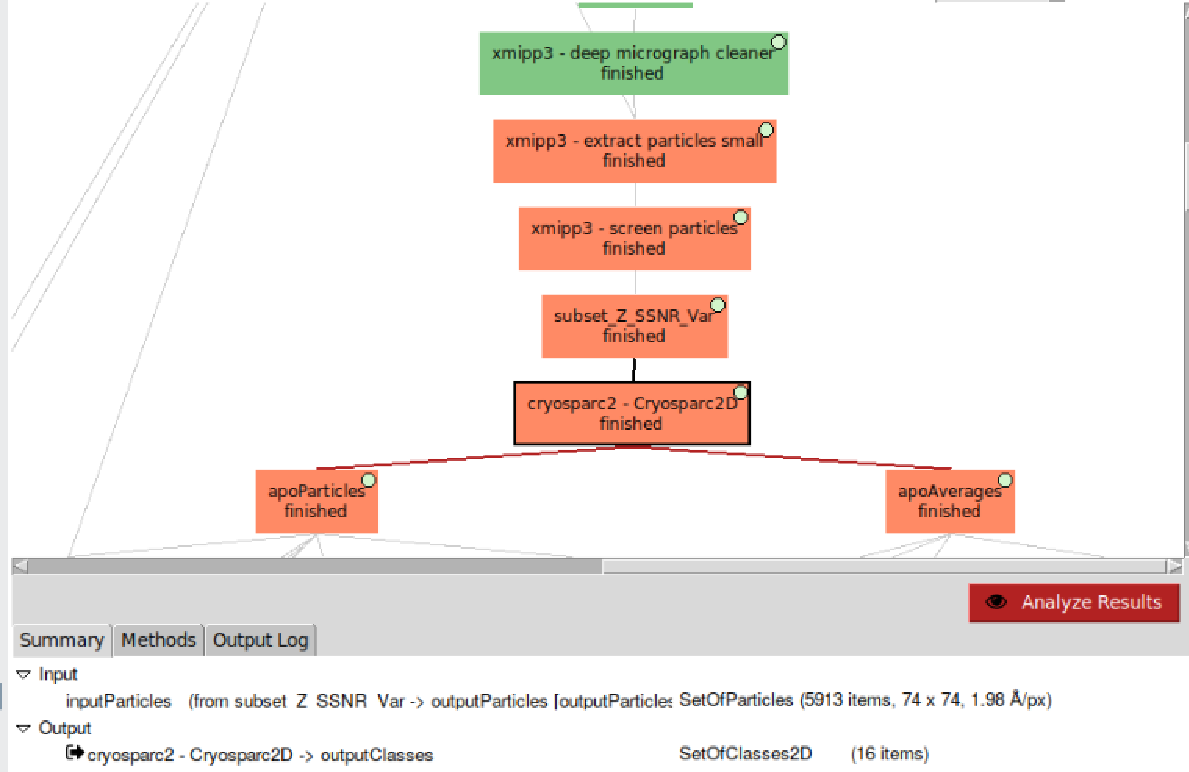
\includegraphics[width=0.95\textwidth]
  {images/cryosparc2_B.pdf}
  \caption{Summary of $cryoSPARC$ \ttt{2D classification} results.}
  \label{fig:cryosparc2_2branches}
  \end{figure}
  
Two branches derive from the \scommand{cryosparc2- 2d classification} protocol box (\ffigure{fig:cryosparc2_2branches}), pointing to two boxes, \ttt{apoParticles} and \ttt{apoAverages}, which include the whole set of particles and the \ttt{2D} classes, respectively. These two branches can be obtained by clicking in the lower part of the Summary (\ttt{cryosparc2 - Cryosparc2D -> outputClasses}). A panel will be displayed with the \ttt{2D} classes. By selecting the classes that we are interested in (14 from 16) and pressing \scommand{Particles}, a new set of 5,673 aligned particles will be created, included in the box \ttt{apoParticles} (see Summary output of the \ffigure{fig:cryosparc2_apoParticles}). 

\begin{figure}[H]
  \centering
  \captionsetup{width=.8\linewidth} 
  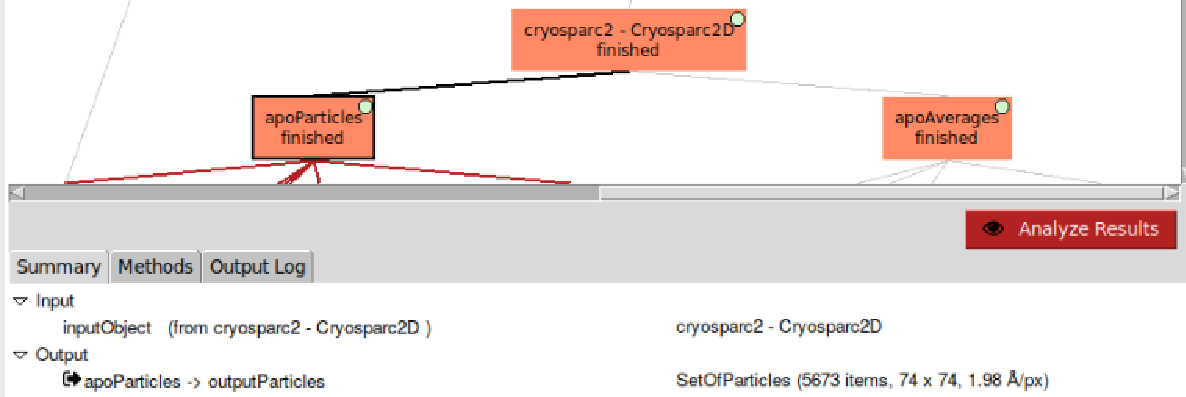
\includegraphics[width=0.95\textwidth]
  {images/cryosparc2_C.pdf}
  \caption{Summary of particle selected in \ttt{apoParticles} box.}
  \label{fig:cryosparc2_apoParticles}
  \end{figure}

If, instead, we press \scommand{Averages}, a new set of 14 class representative particles will be created, included in the box \ttt{apoAverages} (\ffigure{fig:cryosparc2_apoAverages}, Summary output). 

\begin{figure}[H]
  \centering
  \captionsetup{width=.8\linewidth} 
  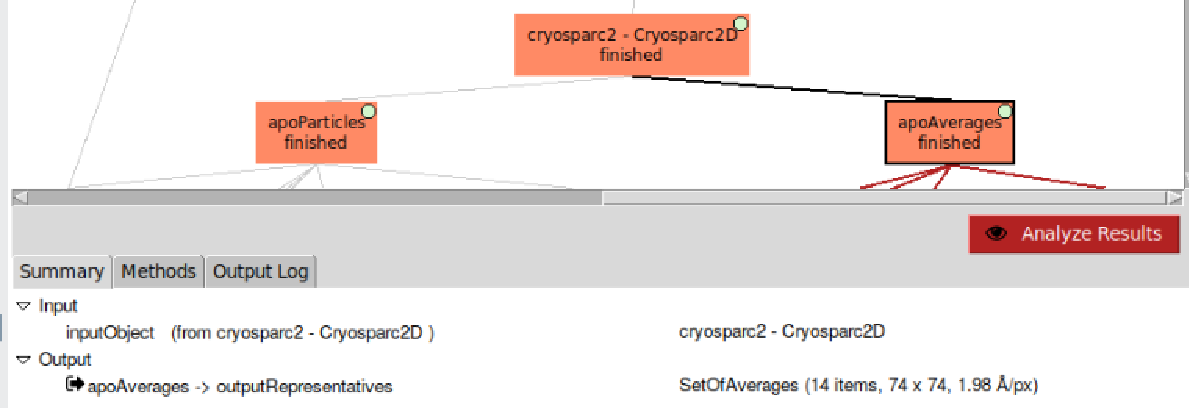
\includegraphics[width=0.95\textwidth]
  {images/cryosparc2_D.pdf}
  \caption{Summary of particle selected in \ttt{apoAverages} box.}
  \label{fig:cryosparc2_apoAverages}
  \end{figure}
  
Finally, if we press \scommand{Classes} after selecting some of the classes, a new set of classes with the number of the selected classes will be created.\\

The selected elements in the two mentioned branches, individual particles and class representative particles, will be used in the next step in the processing workflow to generate the initial volume.  
